% !TeX root = summary.tex
% Preamble
\documentclass[11pt]{article}
\usepackage{graphicx}
\usepackage{url}
\graphicspath{{images/}}

% Packages
\title{Introduction to Networking}
\author{Florian Lotz}
\date{2022}
% Styles:
% BOLD: \textbf{text}
% ITALIC: \textit{text}
% UNDERLINE: \underline{text}

% Document
\begin{document}
\maketitle
\tableofcontents
\pagebreak

\section{Communication Fundamentals}
    All communication methods have three elements in common\
    \begin{itemize}
    \item Sender
    \item Destination
    \item Channel
    \end{itemize}
    Rules or protocols govern all methods of communication.

    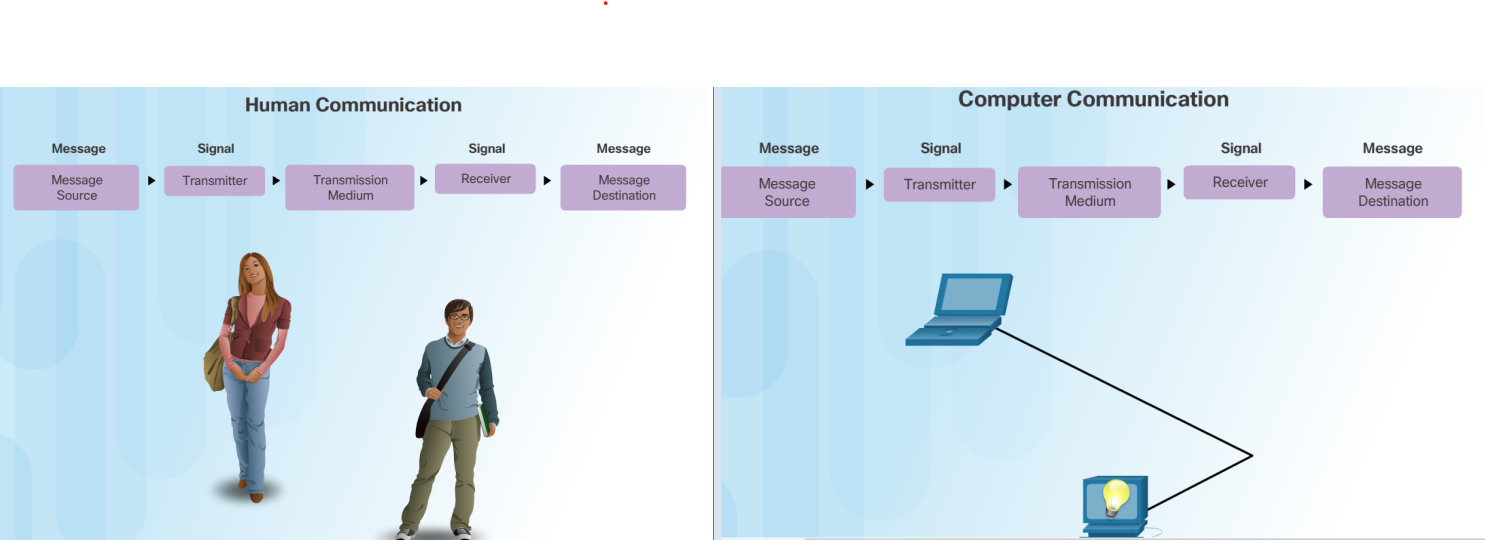
\includegraphics[width=\textwidth]{communication-fundamentals}
\subsection{Rule Establishment}
    Protocols are necessary for effective communication and include:
    \begin{itemize}
    \item An identified sender and receiver
    \item Common language and grammar
    \item Speed and timing of delivery
    \item Confirmation or acknowledgment requirements
    \end{itemize}
    Protocols used in network communications also define:
    \begin{itemize}
    \item Message Encoding
    \item Message Delivery Options
    \item Message Formatting and Encapsulation
    \item Message Timing 
    \item Message Size
    \end{itemize}
    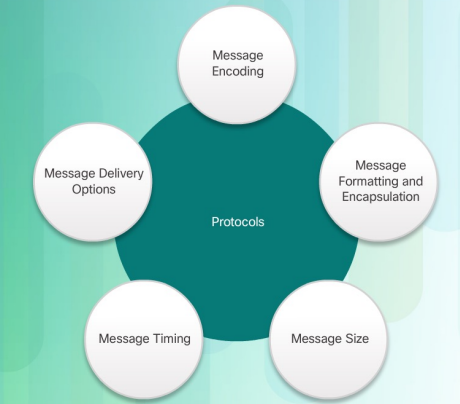
\includegraphics[width=\textwidth]{rule-establishment}
\subsection{Message Encoding}
    \begin{itemize}
        \item Encoding between hosts must be in appropriate format for the medium.
        \item Messages are first converted into bits by the sending host.
        \item Each bit is encoded into a pattern of sounds, light waves, or electrical impulses depending on the network media
        \item The destination host receives and decodes the signals in order to interpret the message.
    \end{itemize}
    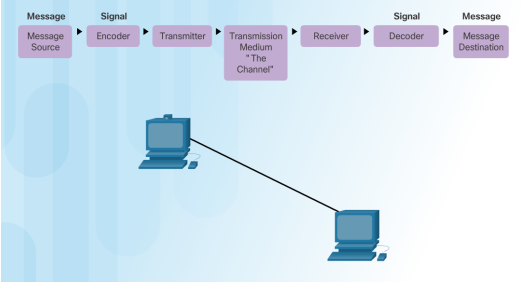
\includegraphics[width=\textwidth]{message-encoding}
\subsection{Message Formatting and Encapsulation}
    \begin{itemize}
        \item There is an agreed format for letters and addressing letters which is required for proper delivery.
        \item Putting the letter into the addressed envelope is called encapsulation.
        \item Each computer message is encapsulated in a specific format, called a frame, before it is sent over the network.
        \item A frame acts like an envelope providing destination address and source address.
    \end{itemize}
    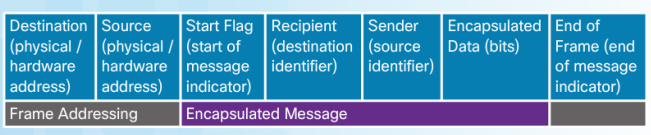
\includegraphics[width=\textwidth]{message-formatting-and-encapsulation}
\subsection{Message Size}
    Humans break long messages into smaller parts or sentences.
    Long messages must also be broken into smaller pieces to travel across a network.
    \begin{itemize}
        \item Each piece is sent in a separate frame.
        \item Each frame has its own addressing information.
        \item A receiving host will reconstruct/combine multiple frames back into the original message.
    \end{itemize}
\subsection{Message Timing}
    \begin{itemize}
        \item Access Method
        Hosts on a network need to know when to begin sending messages and how to respond when collisions occur.
        \item Flow Control
        Source and destination hosts use flow control to negotiate correct timing to avoid overwhelming the destination and ensure information is received.
        \item Response Timeout
        Hosts on the network have rules that specify how long to wait for responses and what action to take if a response timeout occurs.
    \end{itemize}
\subsection{Topology}
    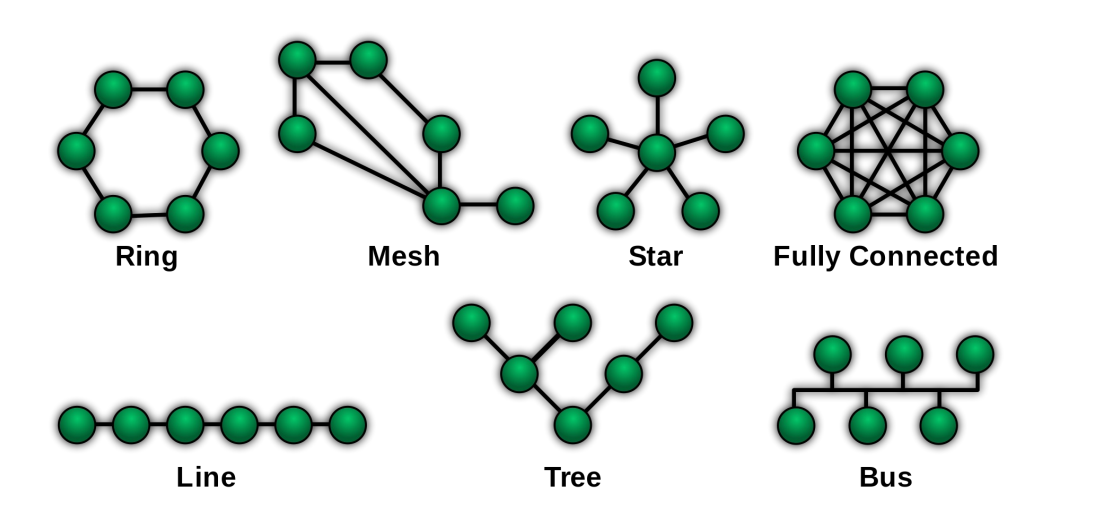
\includegraphics[width=\textwidth]{topology}
    \begin{itemize}
        \item Bus: \\
        Only one station is allowed to send data at a given time.
        Needs mechanism to avoid simultaneous sending resulting in collisions
        \item Ring: \\
        A token travels around a logical ring, regulating the channel access
        \item Star: \\
        Every station is connected to a central node
        Outage of central note implies total outage of whole topology = “Single Point of Failure”
    \end{itemize}
\subsection{(Message) Delivery Options}
    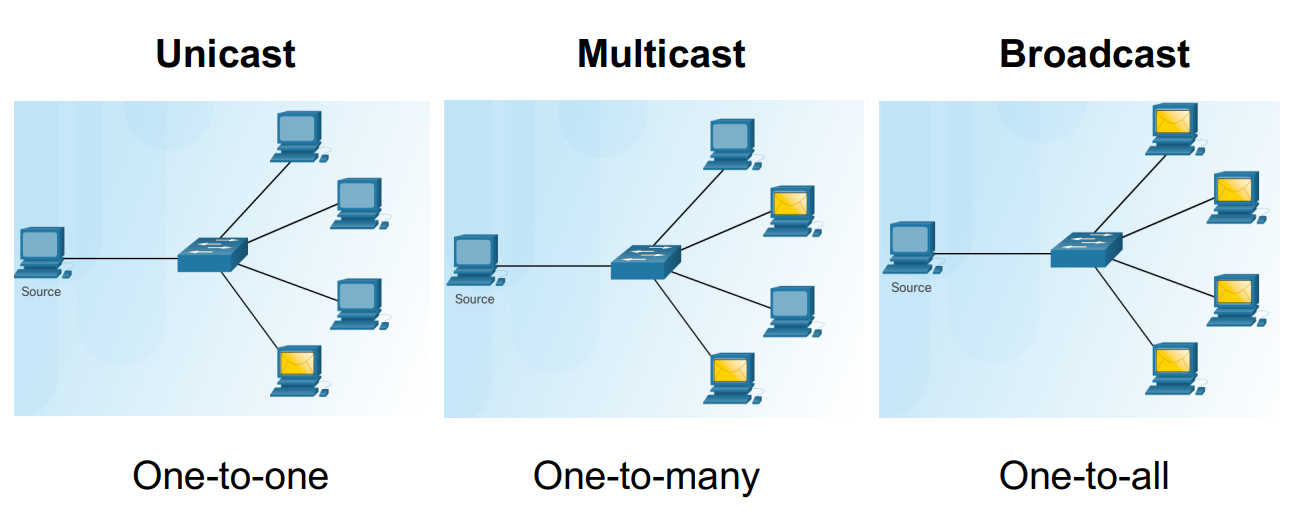
\includegraphics[width=\textwidth]{message-delivery-options}
\subsection{Method of Data Transmission}
    \subsubsection{Circuit Switching}
        One fixed line for the time of communication.
        Disadvantage: waste of bandwidth, there is just a finite number of circuits available
        
        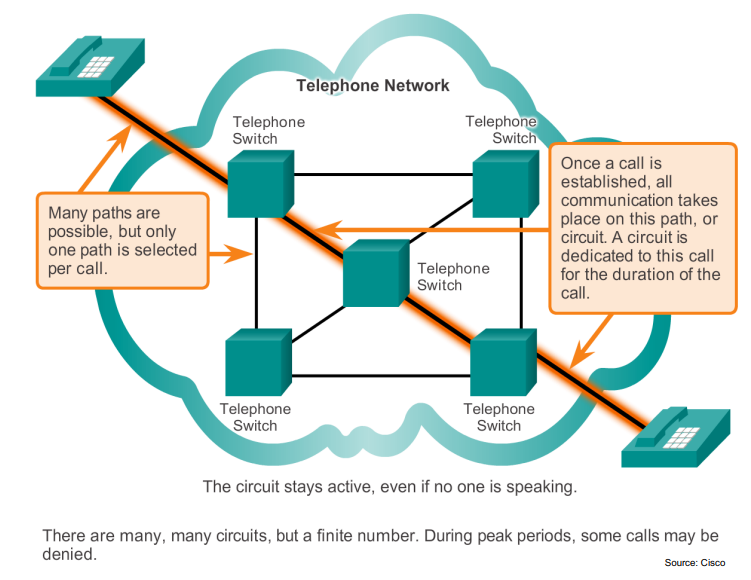
\includegraphics[width=\textwidth]{circuit-switching}
    \subsubsection{Packet Switching}
    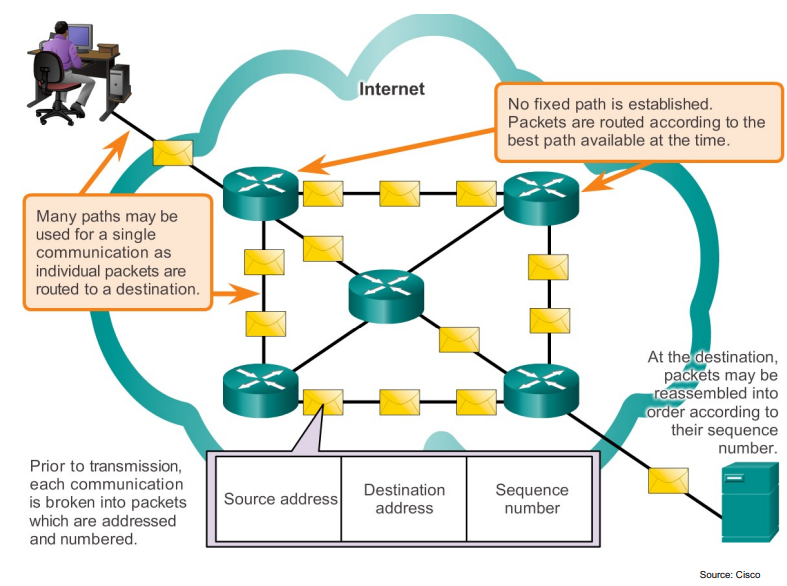
\includegraphics[width=\textwidth]{packet-switching}
    Data is split into several packets (grouped data).
    Every packet is transported through the network separately (order may change due to different paths, delays, etc.).
    Receiver needs to reassemble the packets in their original order.
    “Virtual circuits” emulate circuit switching on a packet-switched network.
\subsection{Performance}
\subsubsection{Bandwidth}
    \begin{itemize}
        \item Theoretical maximum amount of data that can be transmitted.
        \item Measuring unit: bits per second (bits/s).
        \item Bandwidth also exists in the field of signal processing à frequency range between lowest and highest obtainable frequency in Hertz.
    \end{itemize}
    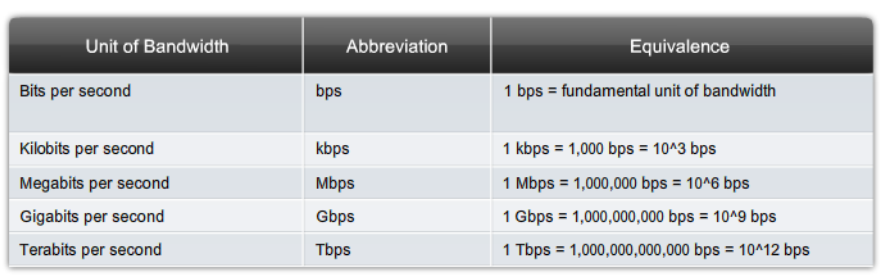
\includegraphics[width=\textwidth]{bandwidth}
\subsubsection{Latency}
    \begin{itemize}
        \item Time of transmission from one node to another
        \item Consist of different delays: the latency of the link, the queuing time, processing time in the components
        \item Round Trip Time (RTT) – amount of time from sending data until receiving the acknowledgment
    \end{itemize}
\subsubsection{Throughput}
    \begin{itemize}
        \item Amount of successful delivered data per time
        \item Depends on Bandwidth and Latency (RTT)
    \end{itemize}
\subsection{Type/Scope}
    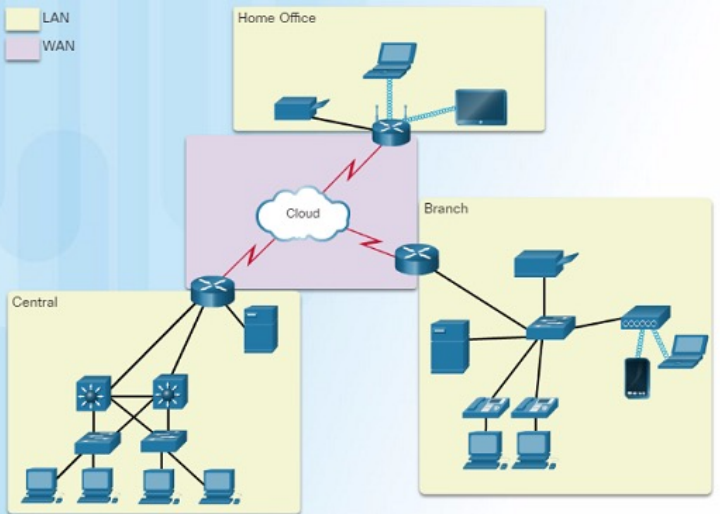
\includegraphics[width=\textwidth]{type-scope}
    \subsubsection{LAN (Local Area Network)}
    spans a small geographic area owned or operated by an individual or IT department
    \subsubsection{WAN  (Wide Area Network) }
    spans a large geographic area typically involving an Internet service provider (ISP)
    \subsubsection{Other types of networks}
    \begin{itemize}
        \item Metropolitan Area Network (MAN)
        \item Wireless LAN (WLAN)
        \item Storage Area Network (SAN)
        \item Personal Area Network (PAN), e.g.: Bluetooth
    \end{itemize}
\subsection{The Internet}
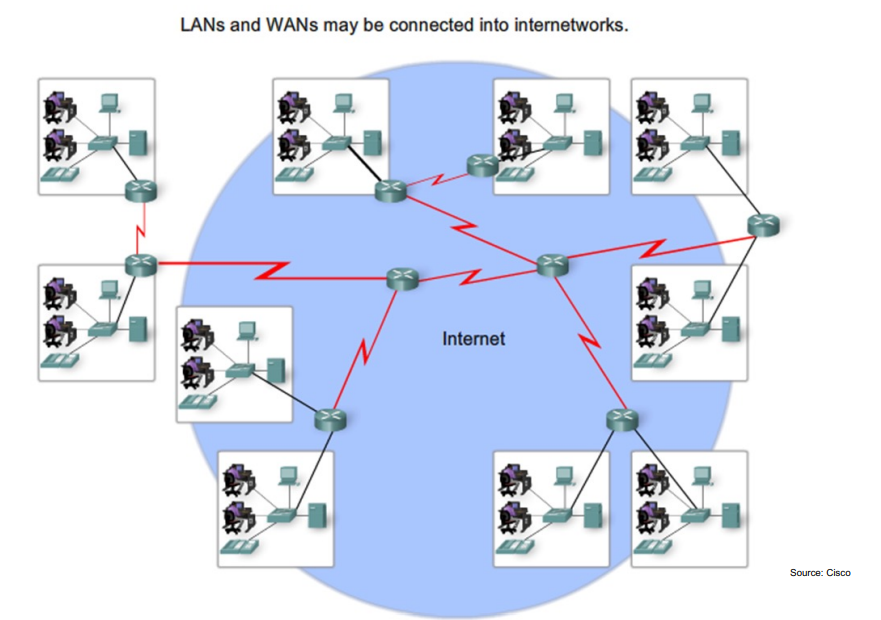
\includegraphics[width=\textwidth]{the-internet}
The purpose of the Internet is to interconnect end systems, called hosts. 
Such as PCs, servers, notebooks, smart phones, etc.
Most hosts that use the Internet are connected to a network, such as a LAN or a WAN.\@
Networks are in turn connected by routers. Each router attaches to two or more networks.
A host may send data to another host anywhere on the Internet:
    \begin{itemize}
        \item The source host breaks the data into a sequence of packets, called IP packets, or IP datagrams.
        \item Each packet includes the unique numeric addresses of the source host and destination host, called IP addresses.
        \item Based on the destination IP address, each packet travels through a series of routers and networks from source to destination.
        \item Each router, upon receiving an IP packet, makes a routing decision and forwards the packet along its way to the destination.
    \end{itemize}
    There is no “component” that is called the “Internet”
    It consists of several LANs and WANs around the world (“A Network of Networks”)
    A network on the Internet is also called Autonomous System (AS)
    \begin{itemize}
        \item An AS may consist of subnetworks
        \item Is managed by a single organization (ISP or large company)
        \item About 90,000 AS are registered by the IANA (Internet Assigned Numbers Authority)
    \end{itemize}
\subsection{How do they interconnect?}
Organizations want to interconnect their networks in a redundant manner
Different strategies:
    \begin{itemize}
        \item Transit: \\
        smaller organizations rent paths through other networks from bigger organizations
        \item Peering: \\
        Organizations make arrangements to exchange data without costs (fair use)
        \item Public Peering Points: \\
        DE – CIX Frankfurt \\
        AT – VIX Vienna 
    \end{itemize}
Biggest providers are called Tier 1 providers

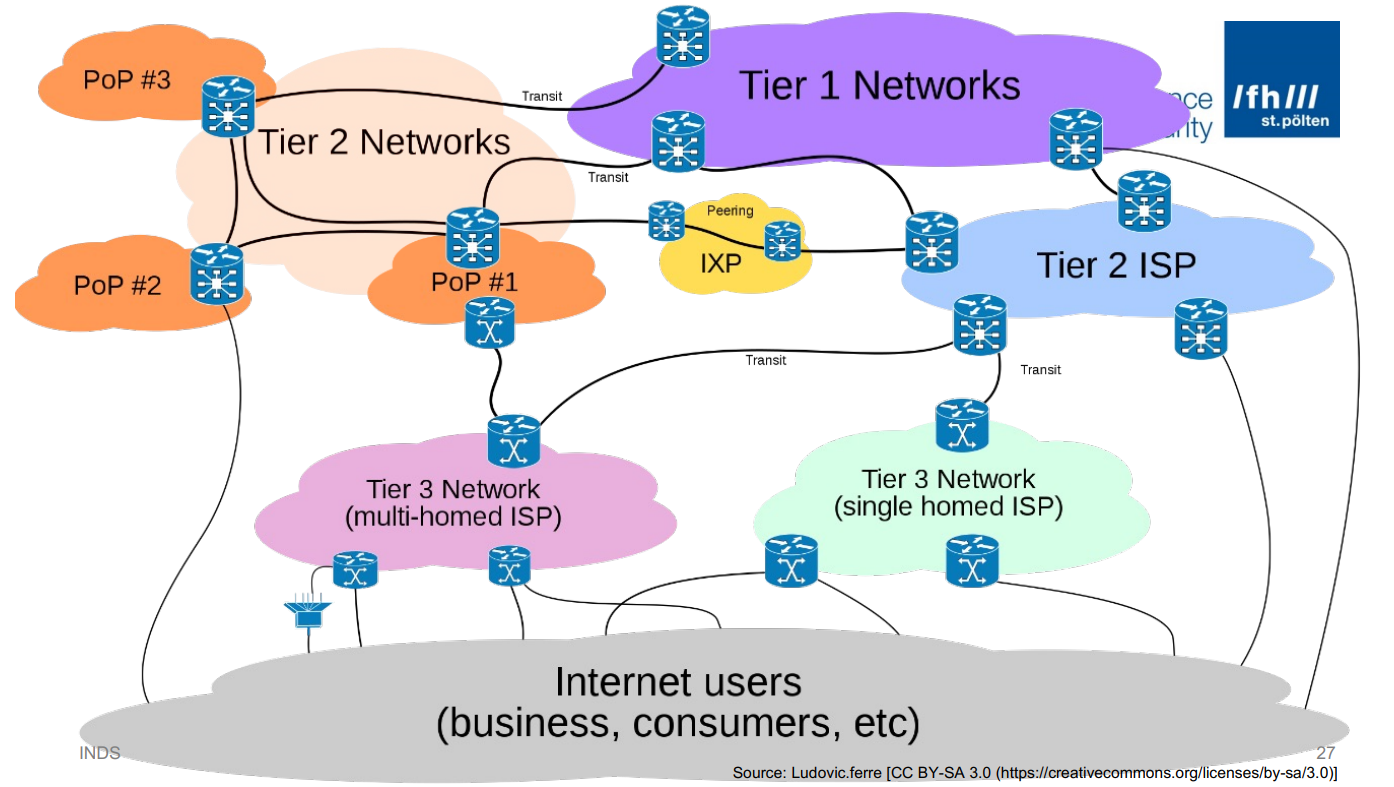
\includegraphics[width=\textwidth]{internet-interconnect}
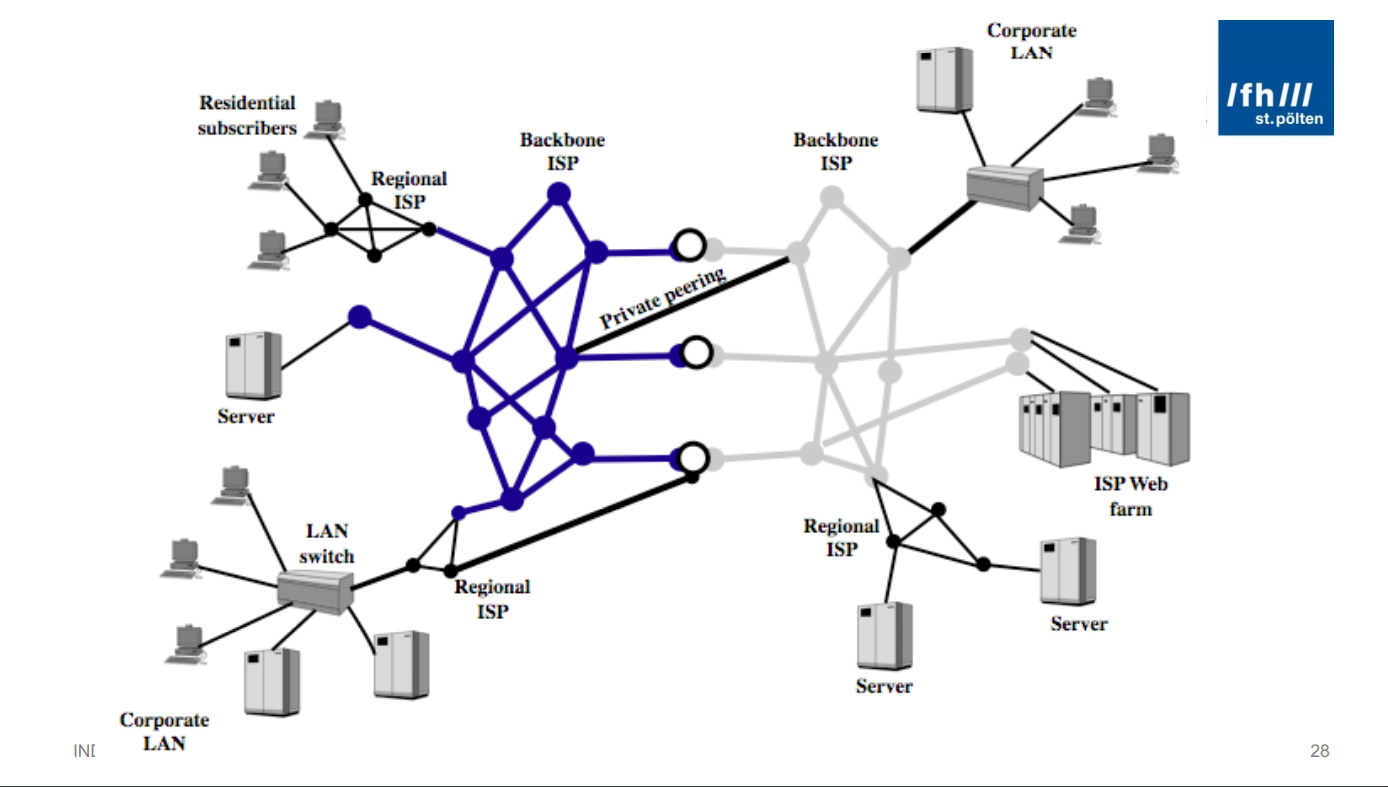
\includegraphics[width=\textwidth]{internet-interconnect-2}
\subsection{History of the Internet}
The first packet switching network and predecessor to todays Internet was the Advanced Research Projects Agency Network (ARPANET), 
which came to life in 1969 by connecting mainframe computers at four locations.
ARPANET was funded by the U.S. Department of Defense for use by universities and research laboratories. 
Bolt, Beranek and Newman (BBN) was the contractor that did much of the initial development of the ARPANET, including creating the first router known as an Interface Message Processor (IMP).
In 1973, Robert Kahn and Vinton Cerf began to work on TCP to develop the next generation of the ARPANET.\@
TCP was designed to replace ARPANETs current Network Control Program (NCP)
In 1978, TCP was divided into two protocols: TCP and IP.\@
Later, other protocols were added to the
TCP/IP suite of protocols including Telnet, FTP, DNS, and many others.
\subsection{How to connect to the Internet}
For Private Use

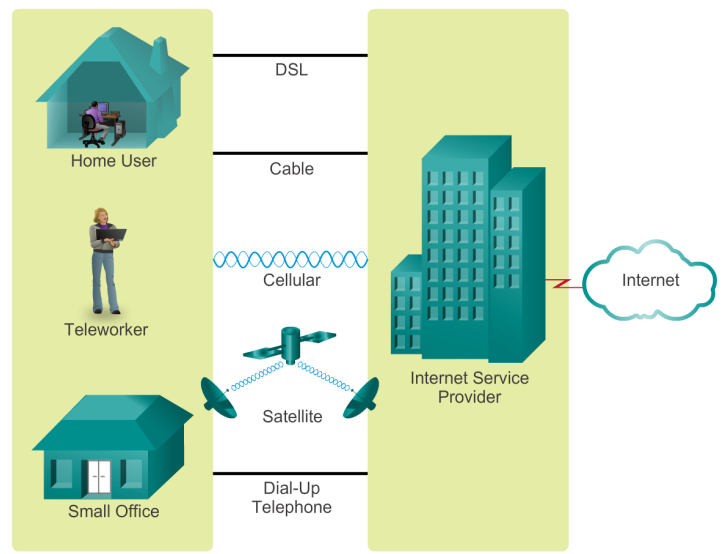
\includegraphics[width=\textwidth]{connect-internet-private-use}

For businesses

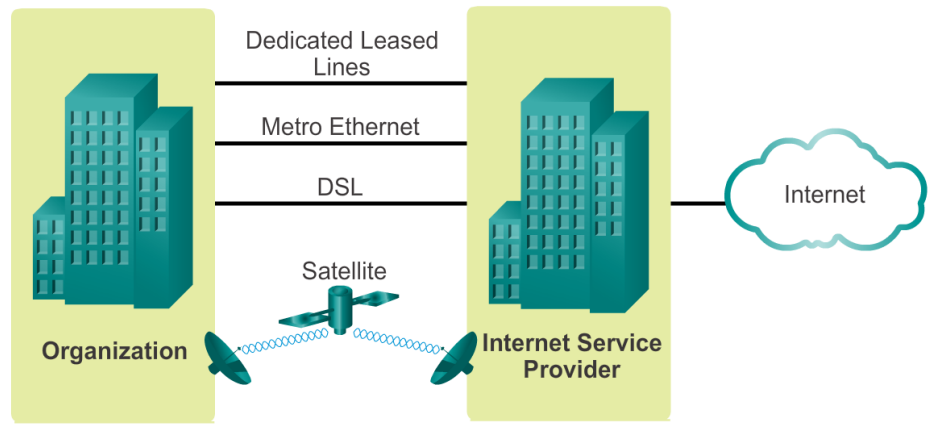
\includegraphics[width=\textwidth]{connect-internet-business-use}
\subsection{Connections between continents}
Submarine cables.
Today only fiber optical cables are used.
\@ First cable was laid in 1851 (copper cable) between France and GB.\@

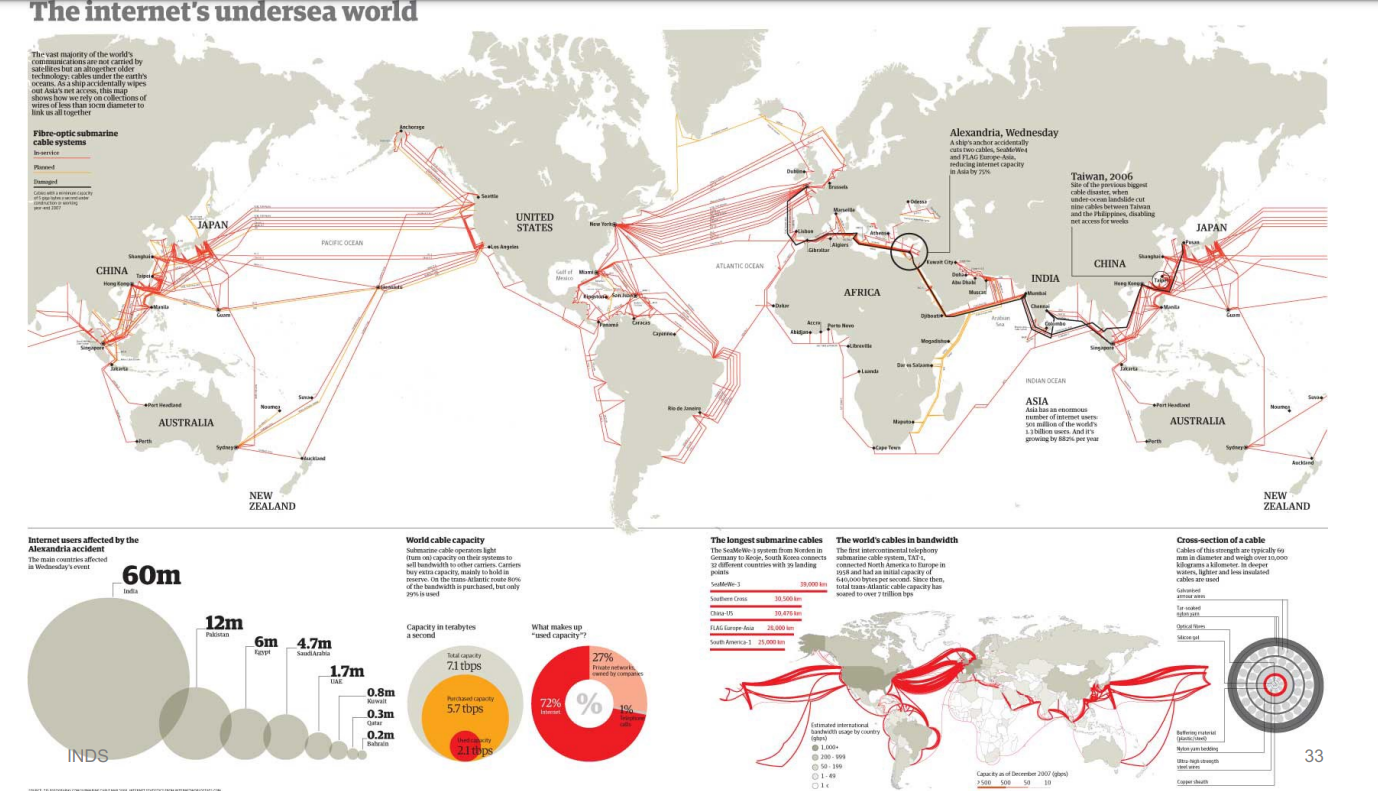
\includegraphics[width=\textwidth]{internet-connections}
\subsection{Paths through the Internet}
\url{https://traceroute-online.com/}
\subsection{Who owns the Internet?}
    \begin{itemize}
        \item Names and addresses are administered by an organization called ICANN (Internet Corporation for Assigned Names and Numbers) \\
        ICANN is a NON-profit organization
        \item IANA (Internet Assigned Numbers Authority) \\
        Department for assigning IP addresses and Names inside the ICANN
        \item The name and address spaces are split up in 5 Regional Internet Registries \\
        these distribute them to Local Internet Registries and ISPs
    \end{itemize}
\subsection{Regional Internet Registries}
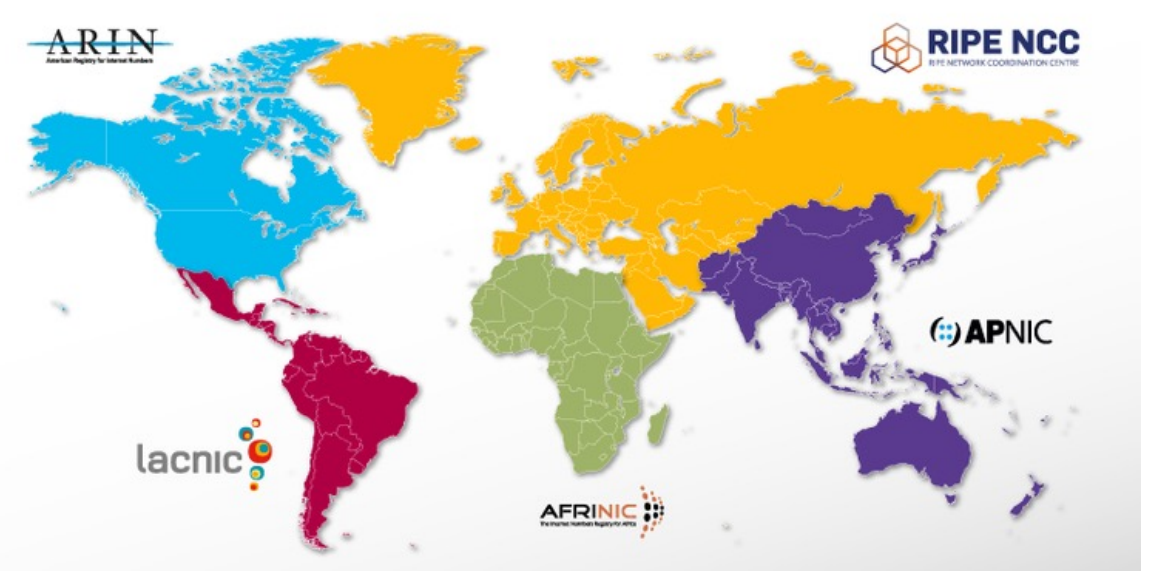
\includegraphics[width=\textwidth]{regional-internet-registries}
\section{Communication Models}
\subsection{Layered Communication Models}
    \begin{itemize}
        \item The communication task is split up in different layers with different functions – “protocol stack”
        \item Layers can only communicate with their neighbors (upper and lower) \\
        Provide “services” for each higher layer
        \item A data unit “travels” through all layers on the sender side (top-down) and then through all layers at the receiver side (bottom-up)
        \item Enhances compatibility: manufacturers have defined interfaces for each layer à following the standards allows compatible devices
    \end{itemize}
\subsection{Benefits of layered models}
\begin{itemize}
    \item Less complex: \\
    Compared to not using a layered model, network models break the concepts into smaller parts/problems.
    \item Standard interfaces \\
    The standard interface definitions between each layer allow multiple vendors to create products that fill a particular role, with all the benefits of open competition
    \item Easier to learn \\
    Humans can more easily discuss and learn about the many details of a protocol
    \item Easier to develop \\
    Reduced complexity allows easier program changes and faster product development.
    \item Multivendor interoperability \\
    Creating products to meet the same networking standards means that computers and networking gear from multiple vendors can work in the same network.
    \item Modular engineering \\
    One vendor can write software that implements higher layers, for example, a web browser, and another vendor can write software that implements the lower layers, for example, Microsoft's built-in TCP/IP software in its OSs.
specification
\end{itemize}
\subsection{OSI Model and TCP/IP Model}
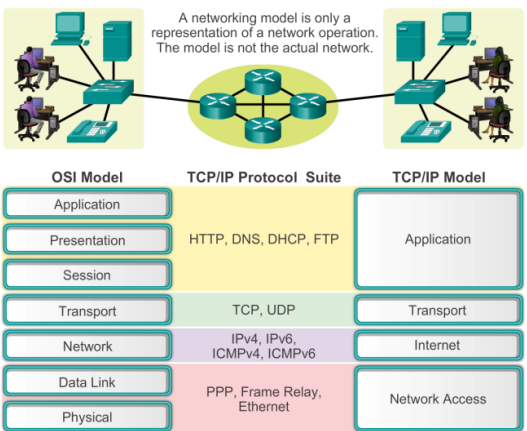
\includegraphics[width=\textwidth]{osi-and-tcp-ip-model}
\subsection{OSI Reference Model}
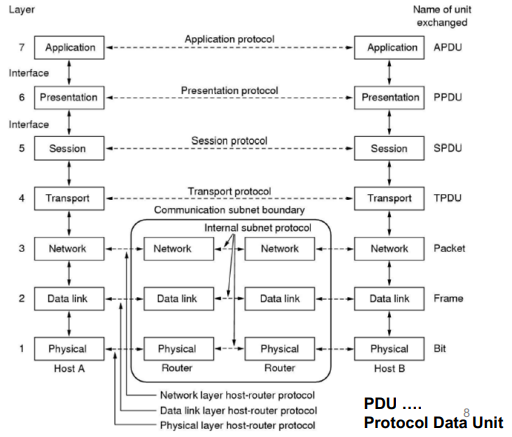
\includegraphics[width=\textwidth]{osi-reference-model}
Open Systems Interconnection (OSI) Reference Model
\begin{itemize}
    \item Standardized Model from the International Standards Organisation (ISO) 
    \item To connect open systems
    \item Consists of 7 Layers
\end{itemize}
\subsection{OSI Layer 1 – Physical Layer}
Transfer of bits over the communication channel
Tasks of the physical layer:
    \begin{itemize}
        \item Voltage level
        \item Signal duration
        \item Pinning / wire map / connectors
        \item Full Duplex / Half Duplex
        \item Transmission medium (copper, fiber, air, …)
    \end{itemize}
\subsection{OSI Layer 2 – Data Link Layer}
\begin{itemize}
    \item Logical link control Layer (LLC)
    \begin{itemize}
        \item Multiplexing for upper layer protocols (IPv4, IPv6, IPX, …)
        \item P2P Flow control (usually not used today, delegated to Layer 4 end-to-end)
    \end{itemize}
    \item Media access control layer (MAC)
    \begin{itemize}
        \item Frame delimiting and recognition
        \item Protection against errors, by generating and checking frame check sequences (FCS)
        \item Channel access mechanism on a shared medium: Carrier Sense Multiple Access (CSMA)
        \item Physical addressing (MAC addresses)
    \end{itemize}
    \item L2 Network Devices: e.g. Switches
\end{itemize}
\subsection{OSI Layer 3 – Network Layer}
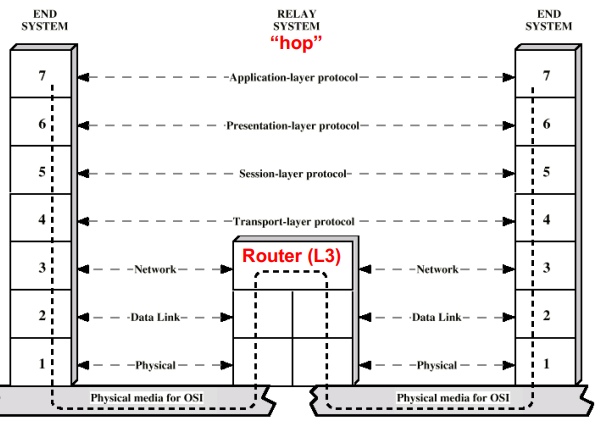
\includegraphics[width=\textwidth]{osi-3-network-layer}
\begin{itemize}
    \item Logical Addressing (e.g. IP addresses)
    \item Route selection for the packets à Chooses the best route
    \begin{itemize}
        \item Routes can be static or dynamic
        \item Routing protocols
    \end{itemize}
    \item Transmission of packets over different networks
    \item L3 Network Devices: e.g. Routers
\end{itemize}
\subsection{OSI Layer 4 – Transport Layer}
\begin{itemize}
    \item Transmits data from sender to receiver independent of the underlying network technologies.
    \begin{itemize}
        \item First End-to-End Layer
        \item Sets up a “connection” between hosts, i.e. \ end-devices / -points / -nodes
    \end{itemize}
    \item Splits the data from the session layer into smaller segments and passes them to the Network Layer
    \item Defines the kind of the service
    \begin{itemize}
        \item Connection-oriented data stream (e.g TCP)
        \item Connectionless data stream (e.g. UDP)
    \end{itemize}
    \item Connection-orientated
    \begin{itemize}
        \item Reliable
        \item Connection management (establishment, transmission, termination)
        \item Error detection
        \item Flow control
        \item Multiplexing (combining two or more data stream into one single physical connection)
    \end{itemize}
    \item Connectionless
    \begin{itemize}
        \item Not reliable
        \item Multiplexing (combining two or more data stream into one single physical connection)
    \end{itemize}
\end{itemize}
\subsection{OSI Layers 5 to 7}
\begin{itemize}
    \item Layers 5 to 7 often combined today in applications
    \item 5: Session Layer
    \begin{itemize}
        \item Provides mechanism for session management between applications
        \item Main purpose is synchronization
    \end{itemize}
    \item 6: Presentation Layer
    \begin{itemize}
        \item Defines the syntax of the transmitted data \\
        ASCII, Unicode, Jpeg, Gif, …
    \end{itemize}
    \item 7: Application Layer \\
    Defines the interface between the application (user) and the network services
\end{itemize}
\subsection{Example Devices and Protocols}
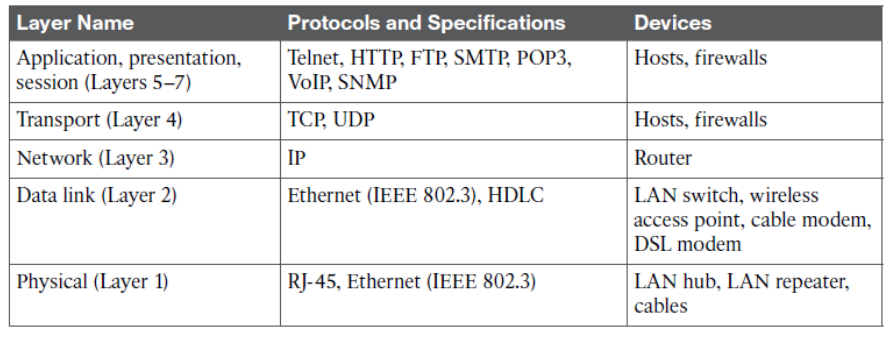
\includegraphics[width=\textwidth]{example-devices-and-protocols}
\subsection{Data transmission through the OSI Layers}
Sender wants to send data to the receiver

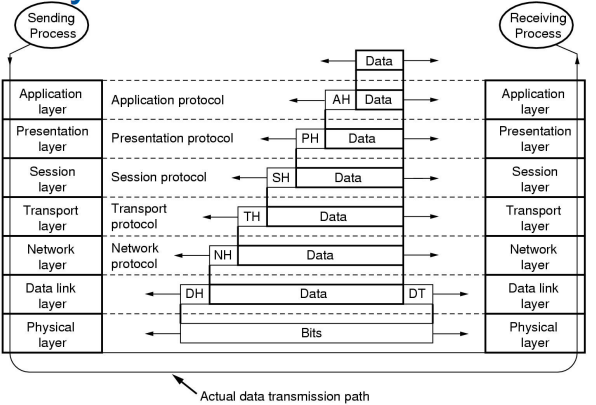
\includegraphics[width=\textwidth]{data-transmission-trhough-osi-layers}
\begin{itemize}
    \item Application Layer generates Data \\
    Passes it to the Presentation Layer and attaches a Header (AH)
    \item \ldots
    \item Network Layer \\
    Adds L3 header: e.g. \ logical addressing and several other fields
    \item Data Link Layer \\
    Adds L2 Header: e.g. \ physical addressing and attaches a checksum at end of frame
    \item Physical Layer \\
    Converts the frame to an electric signal on the wire
\end{itemize}
\subsection{Encapsulation and Segmentation}
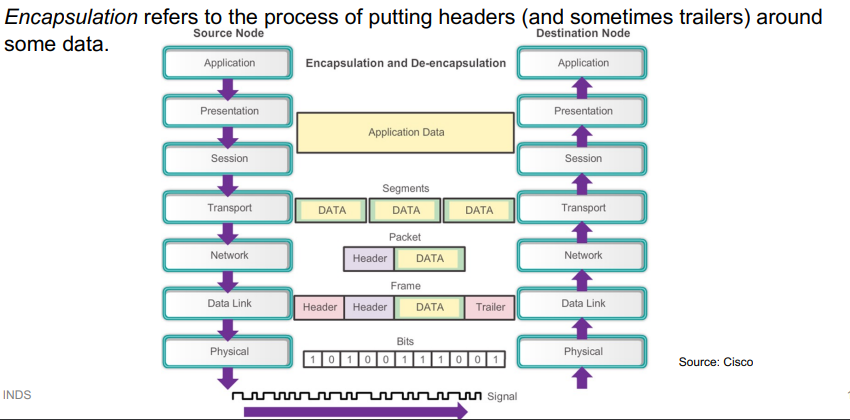
\includegraphics[width=\textwidth]{encapsulation-and-segmentation}

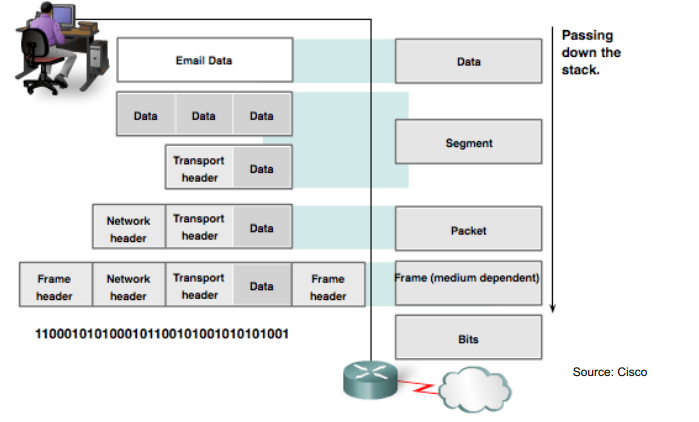
\includegraphics[width=\textwidth]{encapsulation-and-segmentation-2}
\subsection{OSI Layer – Layer Content}
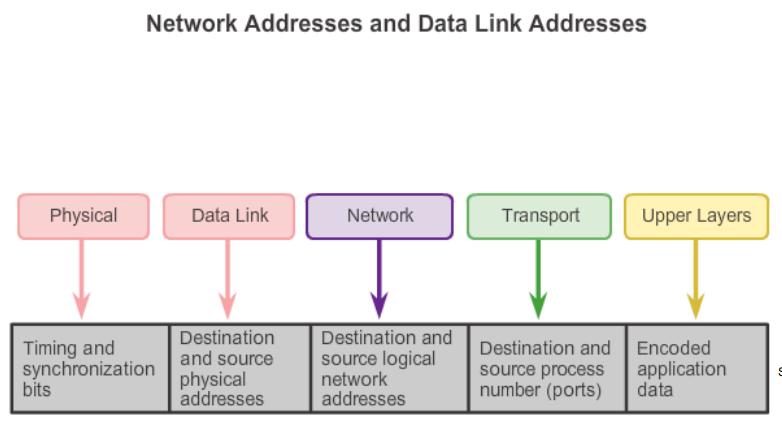
\includegraphics[width=\textwidth]{osi-layer-content}
\subsection{TCP/IP Model}
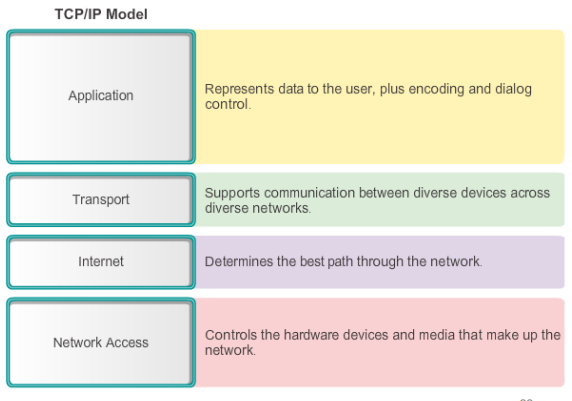
\includegraphics[width=\textwidth]{tcp-ip-model}
\begin{itemize}
    \item Network Access Layer \\
    Combines Layer 1 and Layer 2 of OSI Model (e.g. Ethernet)
    \item Internet Layer
    \begin{itemize}
        \item Transmits packets over different networks to the target
        \item Defines a packet format and a protocol: “Internet Protocol” (IP)
        \item Route selection for the packets à best path selection
    \end{itemize}
    \item Transport Layer
    \begin{itemize}
        \item TCP (Transmission Control Protocol)
        \begin{itemize}
            \item Ensures a reliable and connection-oriented data transmission
            \item Splits the data into numbered packets
            \item Acknowledges received packets
            \item Connection establishment (3 Way Handshake)
        \end{itemize}
        \item UDP (User Datagram Protocol)
        \begin{itemize}
            \item Unreliable and connectionless data transmission
            \item Use for real time applications (voice, video)
        \end{itemize}
    \end{itemize}
    \item Application Layer \\
    Consists of Layer 5 to 7 from the OSI Model
    
    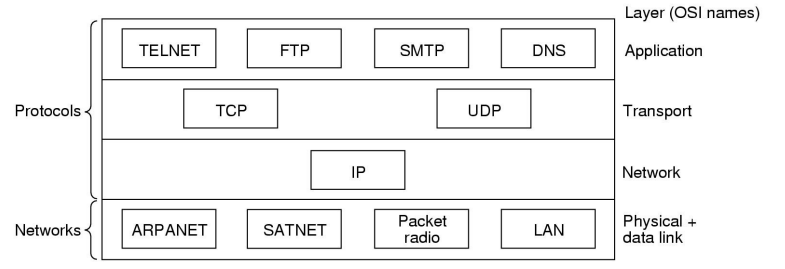
\includegraphics[width=\textwidth]{tcp-ip-application-layer}
\end{itemize}
\begin{itemize}
    \item Simplified Model
    \item Based on the ARPANET
    \item For the packet switched network
    \item Usually operating on IP (L3) and TCP or UDP (L4)
\end{itemize}
\subsection{Comparison OSI and TCP/IP Model}
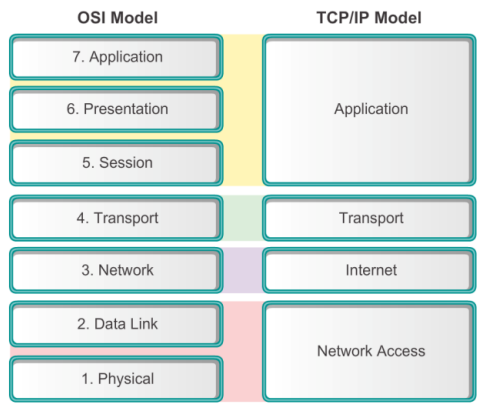
\includegraphics[width=\textwidth]{comparison-osi-tcp-ip-model}
\subsection{Standards}
\begin{itemize}
    \item Internet Society (ISOC) \\
    promotes open development and evolution of Internet use globally.
    \item Internet Architecture Board (IAB) \\
    management and development of Internet standards. 
    \item Internet Engineering Task Force (IETF) \\
    develops, updates, and maintains Internet and TCP/IP technologies.
    \item Internet Research Task Force (IRTF) \\
    focused on long-term research related to Internet and TCP/IP protocols.
    \item Internet Corporation for Assigned Names and Numbers (ICANN) \\
    coordinates IP address allocation and management of domain names.
    \item Internet Assigned Numbers Authority (IANA) \\
    manages IP address allocation, domain name management, and protocol identifiers for ICANN.\@
    \item Request for Comments (RFC) \\
    An RFC document may come from many bodies including from the Internet Engineering Task Force (IETF), the Internet Research Task Force (IRTF), the Internet Architecture Board (IAB), or from independent authors. The RFC system is supported by the Internet Society (ISOC).
    \item Institute of Electrical and Electronics Engineers (IEEE) \\
    dedicated to advancing technological innovation and creating standards in a wide area of industries including networking.
    \item Electronic Industries Alliance (EIA) \\
    standards related to electrical wiring, connectors, and network racks.
    \item Telecommunications Industry Association (TIA) \\
    standards for radio equipment, cellular towers, Voice over IP (VoIP) devices, and satellite communications
    \item International Telecommunications Union-Telecommunication Standardization Sector (ITU-T) \\
    standards for video compression, Internet Protocol Television (IPTV), and broadband communications.
\end{itemize}
\section{Physical Layer}
\subsection{General}
\begin{itemize}
    \item The physical layer is the lowest layer (1) of the OSI 7 layer model 
    \item The various means of (transmission) media as well as the data transmission itself play an important role in this layer
    \item Physical limits must be taken into account when propagating the signals.
\end{itemize}
\subsection{(Simplified) Communications Model}
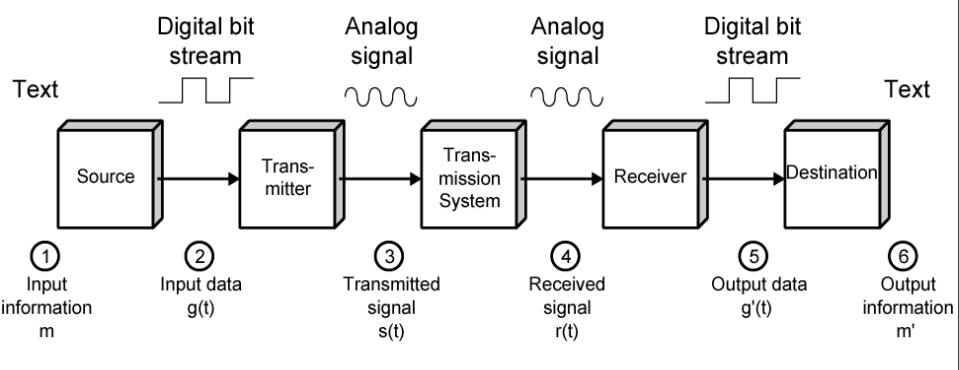
\includegraphics[width=\textwidth]{simplified-comunications-model}
\subsection{Digital Data Transmission}
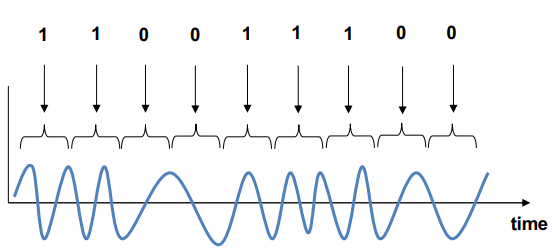
\includegraphics[width=\textwidth]{digital-data-transmission}
\begin{itemize}
    \item Each single bit can be represented by a signal element.
    \item Each signal element takes some time to send.
    \item Bit rate: the number of bits that can be sent out per unit of time.
\end{itemize}
\subsection{What is the objective?}
Maximize the data rate! \\
i.e number of bits that the system can transmit in a unit of time but within an acceptable bit error rate!
The signal received by the receiver is different from the signal sent from the sender \\
Usually, if data rate becomes higher, it is more difficult for the receiver to recognize the signal => higher data rate results in higher bit error rate
\subsection{Terminology}
\begin{itemize}
    \item Data transmission \\
    occurs between transmitter and receiver over some transmission medium.
    \item Signal \\
    electromagnetic waves (Can propagate along the transmission medium)
    \item Transmission Medium
    \begin{itemize}
        \item Guided medium \\
        the signals are guided along a physical path (e.g.\ twisted pair, coaxial cable, optical fiber)
        \item Unguided medium \\
        Wireless (e.g.\ air, water, vacuum)
    \end{itemize}
    \item Direct link \\
    No intermediate devices except amplifiers or repeaters to increase signal strength (applies to both guided and unguided media)
    \item A transmission medium is point-to-point if: \\
    Direct link | Only 2 devices share the medium \\
    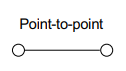
\includegraphics[width=\textwidth]{point-to-point}
    \item A transmission medium is multipoint if: \\
    More than two devices share the same medium \\
    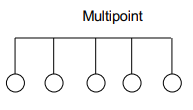
\includegraphics[width=\textwidth]{multipoint}
    \item Simplex transmission \\
    Signals are transmitted in only one direction (e.g.\ Television, Radio)
    \item Half duplex \\
    Signals can be transmitted in either direction, but only one way at a time. (e.g.\ police radio)
    \item Full duplex \\
    Both stations may transmit simultaneously (e.g.\ telephone)
\end{itemize}
\subsection{Signals: Time Domain}
\begin{itemize}
    \item We are concerned with electromagnetic signals used as a means to transmit data. \\
    A signal is generated by the transmitter and transmitted over a medium.
    \item The signal is a function of time, but it can also be expressed as a function of frequency.
    \item Time domain concepts: an electromagnetic signal can be either analog or digital
    \begin{itemize}
        \item Analog signal \\
        Intensity varies in a smooth fashion over time. There is no breaks or discontinuities in the signal
        \item Digital signal \\
        Intensity maintains a constant level for some period of time, then changes to another constant level.
    \end{itemize}
    \item Time domain function of a signal: \( s(t) \) \\
    Specifies the amplitude (in volts) of the signal at each instant in time.
\end{itemize}
\subsection{Analogue and Digital Signals}
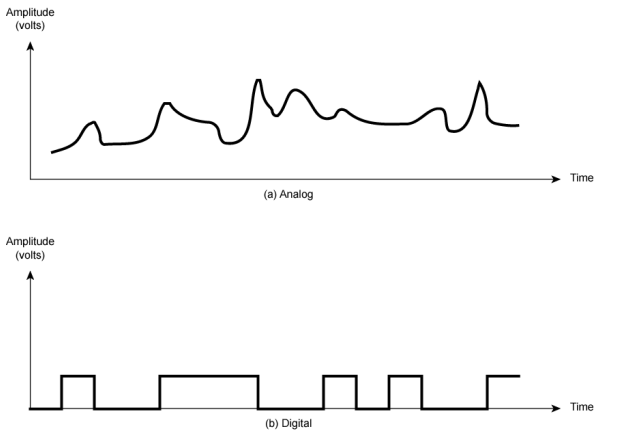
\includegraphics[width=\textwidth]{analog-and-ditigal-signals}
\subsection{Periodic Signals}
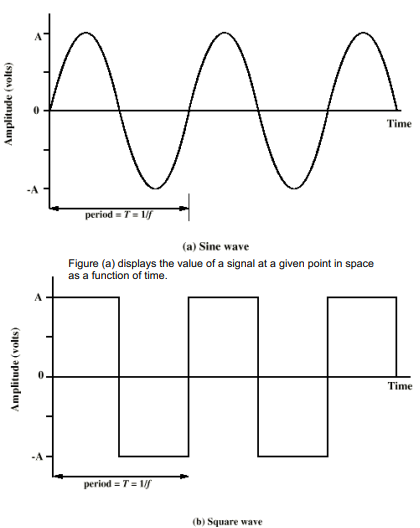
\includegraphics[width=\textwidth]{periodic-signals}
\begin{itemize}
    \item Concept of periodic signal
    \begin{itemize}
        \item The same signal pattern repeats over time.
        \item Otherwise, a signal is aperiodic.
    \end{itemize}
    \item Sine Wave --- represented by three parameters: \\
    \(s(t)= A \sin(2p ft+f)\)
    \item Peak Amplitude (A) \\
    maximum strength of signal, measured in volts
    \item Frequency (f) \\
    \begin{itemize}
        \item Rate of change of signal --- Hertz (Hz) or cycles per second
        \item Period = time for one repetition (T), T = 1/f
    \end{itemize}
    \item Phase (\( \phi \)) \\
    Relative position in time within a single period of a signal
\end{itemize}
\subsection{Frequency}
`Number of repetitive operations per time unit' \\
T --- Period duration \\
\(  f = \frac{1}{T} \)

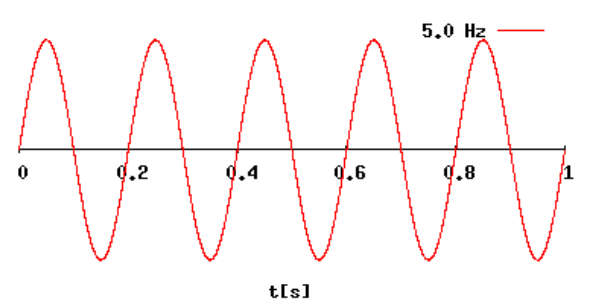
\includegraphics[width=\textwidth]{frequency}i
\begin{itemize}
    \item Typically used for oscillations (e.g.\ pulse frequency of 60 beats per minute)
    \item Unit: Hertz (Hz) = oscillations per second \\
    \(  1 Hz = \frac{1}{s} = s^{-1} \) \\
    \(  1 kHz = 1,000 Hz \) \\
    \(  1 MHz  = 1,000 kHz = 1,000,000 Hz \) \\
    \(  1 GHz  = 1,000,000 kHz = 1 billion Hz \)
\end{itemize}
\subsection{Amplitude}
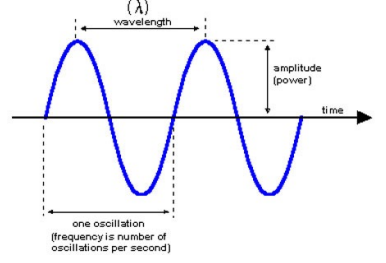
\includegraphics[width=\textwidth]{amplitude}
\begin{itemize}
    \item “maximum deflection of a wave”
    \item The amplitude corresponds to signal strength
    \item Hence, attenuation means a reduction of the amplitude.
\end{itemize}
\subsection{Amplitude}
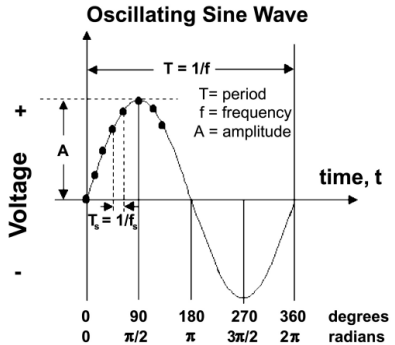
\includegraphics[width=\textwidth]{phase-1}

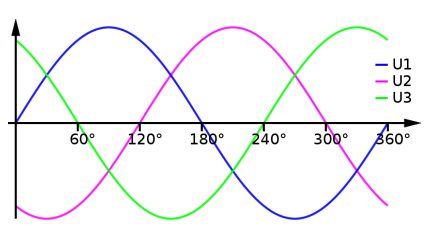
\includegraphics[width=\textwidth]{phase-2}

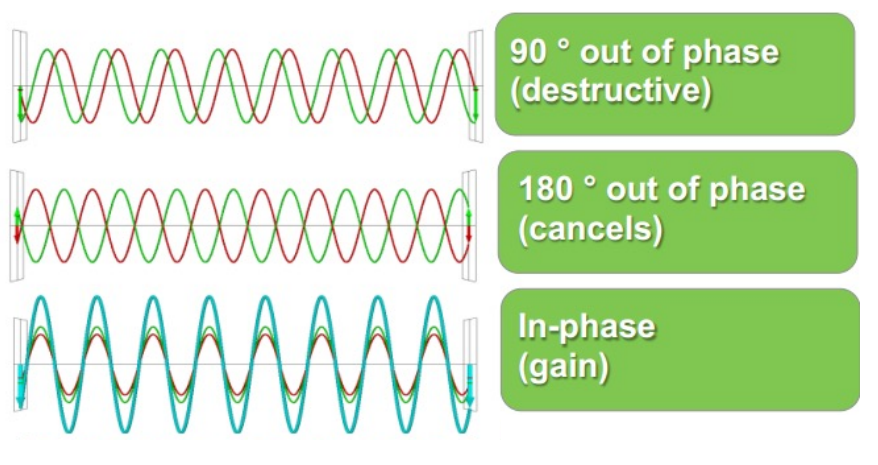
\includegraphics[width=\textwidth]{phase-3}
\begin{itemize}
    \item describes the correlation of two signals
    \item in degrees, where 360° corresponds to a whole cycle / period
    \item Phase shift is the distance between the peak values of two signals of the same frequency
\end{itemize}
\subsection{Interference}
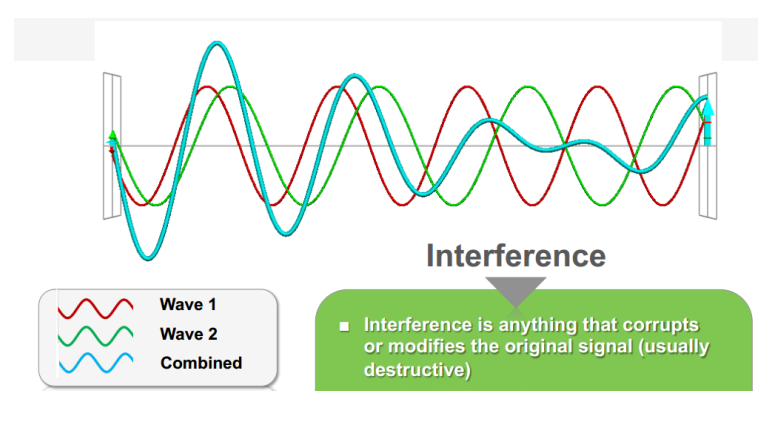
\includegraphics[width=\textwidth]{interference}
\subsection{Varying Sine Waves}
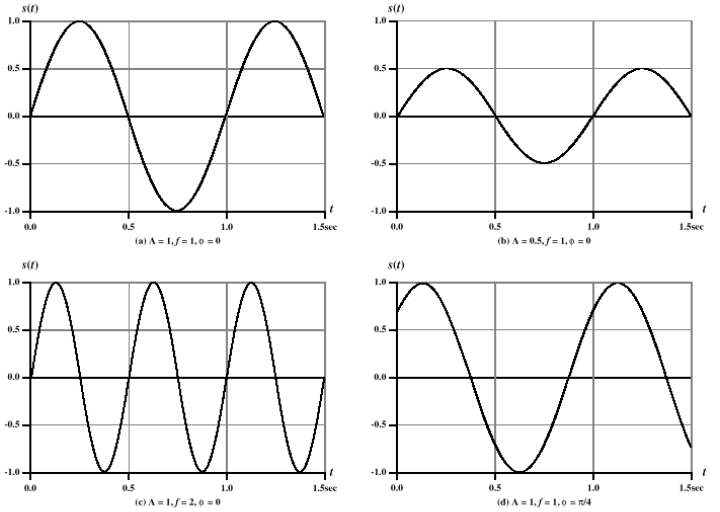
\includegraphics[width=\textwidth]{varying-sine-waves}
\subsection{Signals: Frequency Domain}
\begin{itemize}
    \item In practice, an electromagnetic signal will be made up of many frequencies. \\
    A frequency means a pure sine wave
    \item It can be shown (by Fourier analysis) that any signal is made up of components at various frequencies, in which each component is a sinusoid.
    \begin{itemize}
        \item By adding together enough sinusoidal signals, each with the appropriate amplitude, frequency, and phase, any electromagnetic signal can be constructed.
        \item Any electromagnetic signal can be shown to consist of a collection of periodic analog signals (sine waves) at different amplitudes, frequencies, and phases
    \end{itemize}
    \item Frequency domain function of a signal:  \( S(f) \) \\
    Specifies the peak amplitude of the constituent frequencies of the signal.
\end{itemize}
\subsection{Addition of Frequency Components}
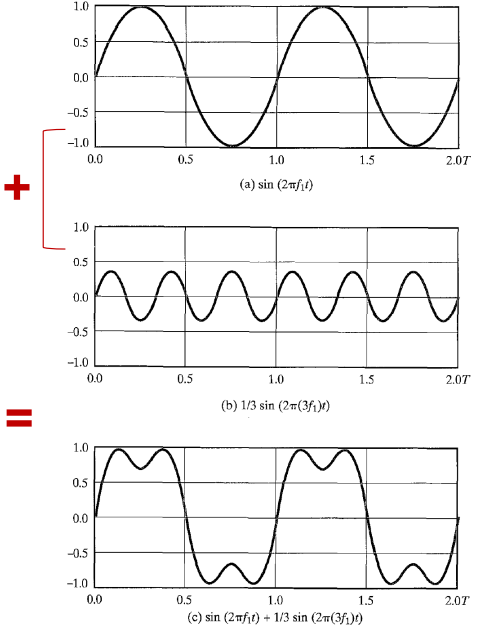
\includegraphics[width=\textwidth]{addition-of-frequency-components}
Signal (c) has only two frequency components:
\begin{itemize}
    \item (a) frequency f
    \item (b) frequency 3f
\end{itemize}
\subsection{Frequency Domain}
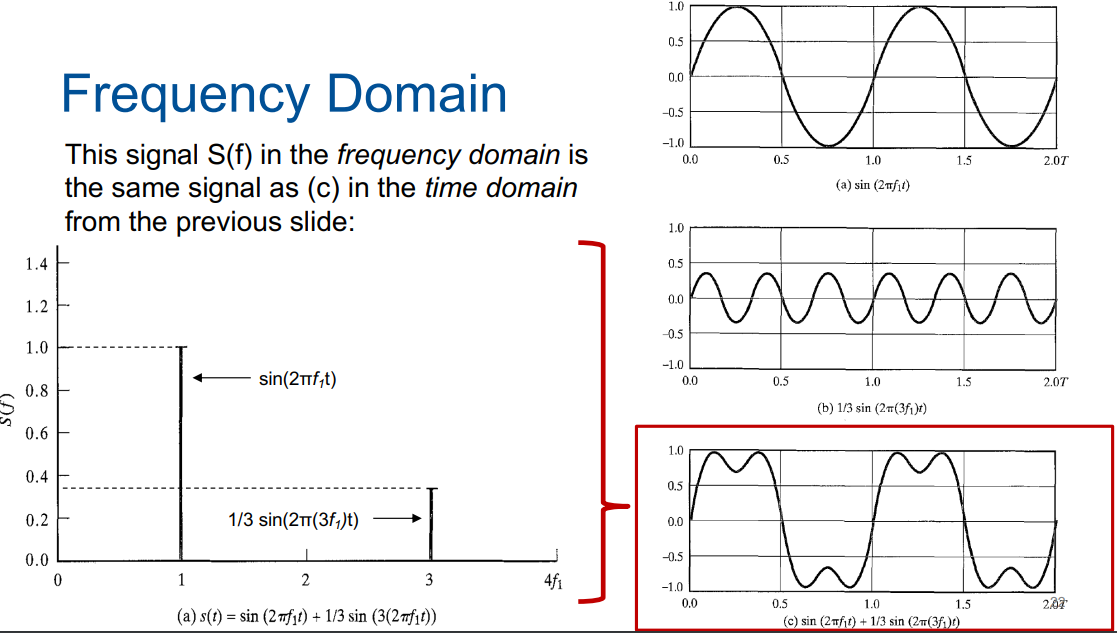
\includegraphics[width=\textwidth]{frequency-domain.png}

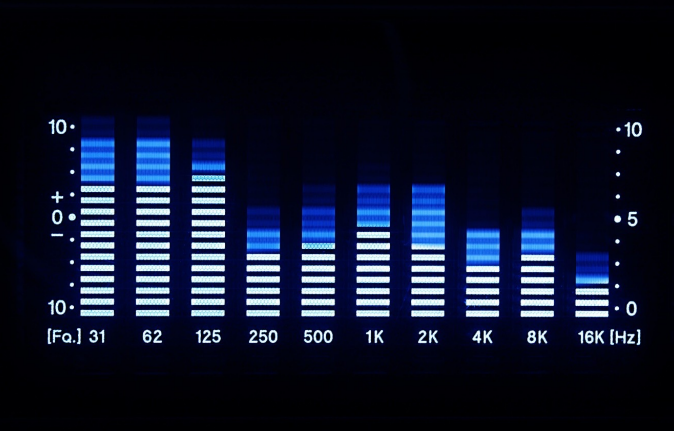
\includegraphics[width=\textwidth]{frequency-domain-2.png}
\subsection{Fourier Analysis}
\begin{itemize}
    \item The French mathematician Jean Baptiste Joseph Fourier (1768\-1830) proved the following connection: \\
    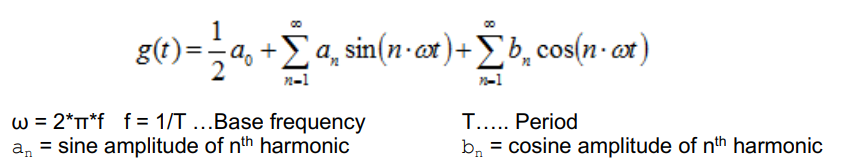
\includegraphics[width=\textwidth]{fourier-analysis.png}
    \item Such a decomposition is called a Fourier series
    \item In simple terms à each periodic signal can be decomposed into a sum of sine and cosine oscillations
    \item A data signal with a finite duration can be imagined in such a way that the same pattern is repeated endlessly with a period duration of \( T \)
    \item The factors are calculated as follows: \\
    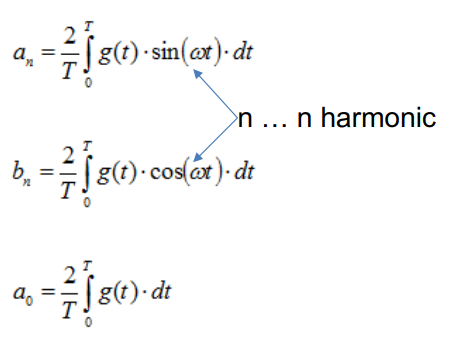
\includegraphics[width=\textwidth]{fourier-analysis-1.png}

    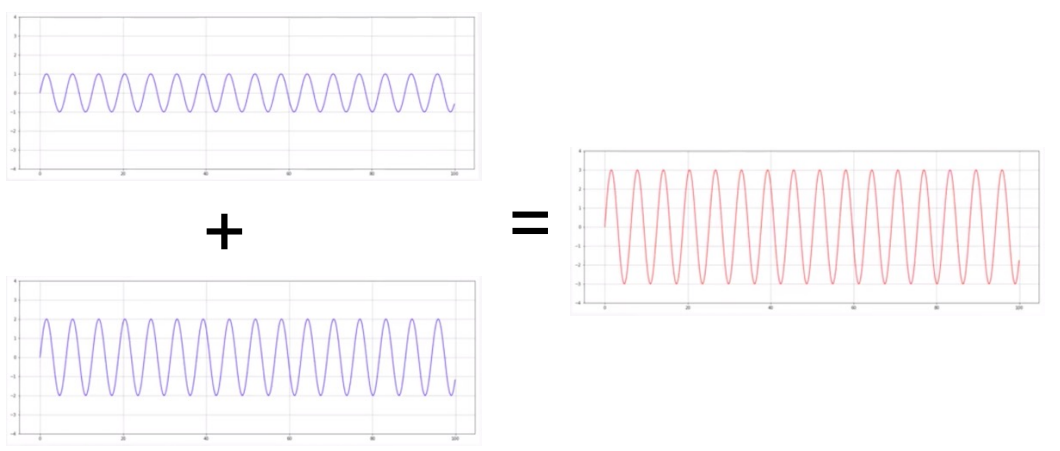
\includegraphics[width=\textwidth]{fourier-analysis-2.png}

    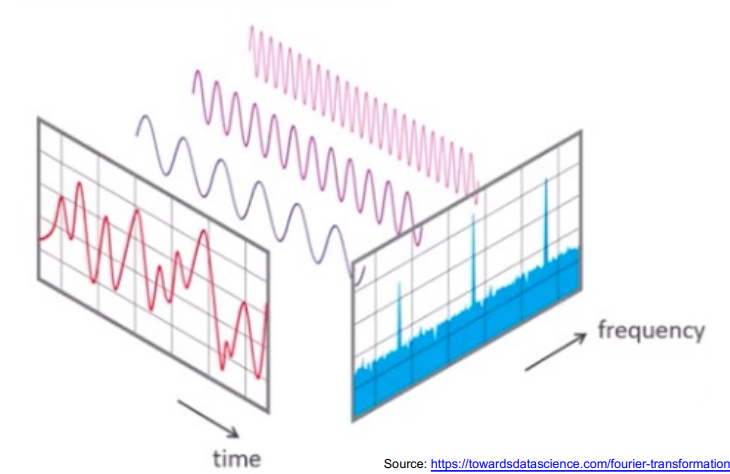
\includegraphics[width=\textwidth]{fourier-analysis-3.png}

    \item Amplitudes of the individual signals and the dependence of the total signal on the available bandwidth: \\
    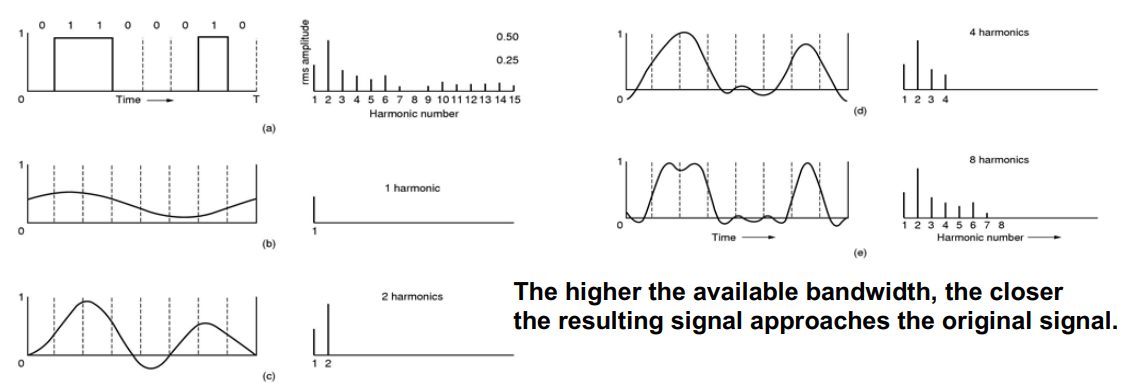
\includegraphics[width=\textwidth]{fourier-analysis-4.png}
    \item In general, any digital waveform will have infinite bandwidth \\
    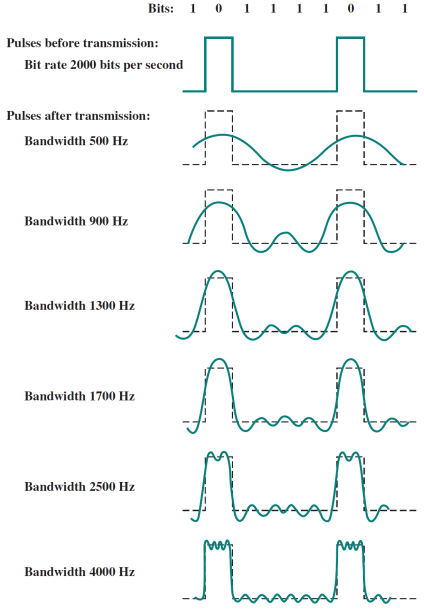
\includegraphics[width=\textwidth]{fourier-analysis-5.png}
    \item If we attempt to transmit this waveform as a signal over any medium, the transmission system will limit the bandwidth that can be transmitted.
    \item Economic and practical reasons dictate that digital information be approximated by a signal of limited bandwidth.
    \item Limiting the bandwidth creates distortions, which makes the task of interpreting the received signal more difficult.
    \item The more limited the bandwidth, the greater the distortion, and the greater the potential for error by the receiver.
    \item If the data rate of the digital signal is \(W bps\), then a very good representation can be achieved with a bandwidth of \(2W Hz\).
    \item The higher the data rate of a signal, the greater is the bandwidth required for transmission.
\end{itemize}

\includegraphics[width=\textwidth]{fourier-analysis-6}

\includegraphics[width=\textwidth]{fourier-analysis-7}

\includegraphics[width=\textwidth]{fourier-analysis-8}

\begin{itemize}
    \item The time \(T\) required to transmit e.g.\ the ASCII letter “N” depends both on the coding method and on the signal frequency
    \item Signal frequency: how often per second the signal changes its value (voltage) (Measured in Hertz (Hz))
    \item 8 bit encoded ASCII character (e.g.: N => 01001110) \\
    \includegraphics[width=\textwidth]{fourier-analysis-9.png}
\end{itemize}

\includegraphics[width=\textwidth]{fourier-analysis-10.png}

\includegraphics[width=\textwidth]{fourier-analysis-11.png}

\includegraphics[width=\textwidth]{fourier-analysis-12.png}

\subsection{Spectrum and Bandwidth}
\begin{itemize}
    \item Spectrum of a signal (the range of frequencies contained in the signal)
    \item Absolute bandwidth of a signal (the width of the signal spectrum) \\
    Many signals have an infinite bandwidth!
    \item Effective bandwidth of a signal (often just referred to as bandwidth) \\
    the narrow band of frequencies containing “most” of the signal energy
    \item DC Component (dc: direct current)
    \begin{itemize}
        \item the component of zero frequency (i.e., \(f = 0\))
        \item With no dc component, a signal has an average amplitude of zero.
        \item With a dc component, a signal has a frequency term at \(f = 0\) and a nonzero average amplitude.
    \end{itemize}
\end{itemize}
\subsection{Signal with DC Component}
\includegraphics[width=\textwidth]{signal-with-dc-component}
\subsection(Frequency Components of Square Wave)
\includegraphics[width=\textwidth]{frequency-components-of-square-wave}
\subsection{Data Rate and Bandwidth}
\begin{itemize}
    \item Effective bandwidth is the band within which most of the signal energy is concentrated. Here, “most” is somewhat arbitrary.
    \item Although a given waveform may contain frequencies over a very broad range, as a practical matter, any transmission system will be able to accommodate only a limited band of frequencies.
    \begin{itemize}
        \item because of the limitation of transmitter and medium and receiver
        \item This limits the data rate that can be carried on the transmission system.
    \end{itemize}
\end{itemize}
\subsection{Effective Bandwidth}
\begin{itemize}
    \item Effective bandwidth is one property of a transmission system.
    \item If the effective bandwidth of the input signal is larger than the bandwidth of transmission system, the output signal will be distorted a lot!
    \item The signal’s bandwidth should match the bandwidth supported by the transmission system.
\end{itemize}

\includegraphics[width=\textwidth]{transmission-system}
\subsection{Analog and Digital Data Transmission}
The two terms “analog” and “digital” are used in the following three contexts:
\begin{itemize}
    \item Data (Entities that convey meaning or information)
    \item Signals (electromagnetic representations of data)
    \item Transmission (The communication of data by the propagation and processing of signals)
\end{itemize}
Analog: continuous \\
Digital: discrete
\subsection{Analog vs. Digital Data}
\begin{itemize}
    \item Analog data \\
    Continuous values within some interval (Represented by real numbers)
    \item Digital data \\
    Discrete values, e.g., text, integers
    \item Computers use digital data
    \begin{itemize}
        \item Even double precision floating numbers are discrete!
        \item In practice, digital data are used to approximate analog data, e.g.\ \\
        brightness of color can be represented by 0, 1, …, 255 \\
        loudness of sound can be represented by 0, 1, …, 255
        \item Digital data are stored as bit stream in computers.
    \end{itemize}
    \item In a communication system, data are propagated by means of electromagnetic signals
    \item Analog signal
    \begin{itemize}
        \item Propagated over a variety of media: wire, fiber optic, air
        \item Continuously varying according to the source information
        \begin{itemize}
            \item Speech bandwidth: \(\tilde 100Hz\) to \(\tilde 7kHz\)
            \item Video bandwidth: \(\tilde 4MHz\)
        \end{itemize}
    \end{itemize}
    \item Digital signal
    \begin{itemize}
        \item A sequence of voltage pulses
        \item Almost unlimited bandwidth
    \end{itemize}
\end{itemize}
\subsection{Digital Signals}
\begin{itemize}
    \item Generally cheaper than analog signaling
    \item Less susceptible to noise
    \item BUT:\ Suffer more from attenuation! \\
    Pulses become rounded and smaller à Leads to loss of information \\
    \includegraphics[width=\textwidth]{digital-signals.png}

\end{itemize}
\subsection{Bit Stream to Digital Signal}
\includegraphics[width=\textwidth]{bit-stream-to-digital-signal}
User input at a PC is converted into a stream of binary digits (1s and 0s). \\
In this graph of a typical digital signal, binary one is represented by +5 volts and binary zero is represented by -5 volts. \\
The signal for each bit has a duration of 0.02 msec, giving a data rate of 50,000 bits per second (50 kbps). \\ 
\subsection{Data and Signals}
\begin{itemize}
    \item Usually, we use digital signals for digital data and analog signals for analog data
    \item Analog data are a function of time and occupy a limited frequency spectrum (Can be represented by an electromagnetic signal occupying the same spectrum.)
    \item Digital data can be represented by digital signals, with a different voltage level for each of the two binary digits.
    \item Analog signal can carry digital data
    \begin{itemize}
        \item Modem: modulator/demodulator
        \item The modem converts a series of binary voltage pulses into an analog signal by encoding the digital data onto a carrier frequency.
    \end{itemize}
    \item Digital signal can carry analog data
    \begin{itemize}
        \item Codec (coder-decoder): the codec takes an analog signal that directly represents e.g.\ voice data and approximates that signal by a bit stream. At the receiving end, the bit stream is used to reconstruct the analog data.
    \end{itemize}
\end{itemize}
\subsection{Analog Signals Carrying Analog and Digital Data}
\includegraphics[width=\textwidth]{analog-signals-carrying-analog-and-digital-data}

\includegraphics[width=\textwidth]{analog-signals-carrying-analog-and-digital-data-1.png}
\subsection{Analog Transmission}
Analog transmission = transmitting analog signals without regard to their content \\
\begin{itemize}
    \item The signals may represent analog or digital data.
    \item In either case, the analog signal will become weaker after a certain distance
    \item Analog transmission system includes amplifiers to boost the energy in the signal.
    \item Unfortunately, the amplifier also amplifies noise.
    \item With amplifiers cascaded for long distances, signal becomes more and more distorted
    \begin{itemize}
        \item For analog data e.g.\ a voice, a bit of distortion can be tolerated, and data remain intelligible
        \item For digital data, cascaded amplifiers will introduce bit errors!
    \end{itemize}
\end{itemize}
\subsection{Digital Transmission}
\begin{itemize}
    \item Digital transmission is concerned with the content of the signal. \\
    It can use digital signal, or analog signal.
    \item Repeaters are used instead of amplifiers \
    \begin{itemize}
        \item A repeater receives the signal, recovers the pattern of 1s and 0s, regenerates the signal, and retransmits the signal.
        \item Amplifiers cannot do this, as the signal has no meaning of 0 or 1
    \end{itemize}
    \item Attenuation is overcome, noise is not cumulative
\end{itemize}
\subsection{Transmission Impairments}
With any communications system, the signal that is received may differ from the signal that is transmitted, due to various transmission impairments. \\
\begin{itemize}
    \item Consequences
    \begin{itemize}
        \item For analog signals: degradation of signal quality
        \item For digital signals: bit error
    \end{itemize}
    \item The most significant impairments include:
    \begin{itemize}
        \item Attenuation and attenuation distortion
        \item Delay distortion
        \item Noise
    \end{itemize}
\end{itemize}
\subsection{Attenuation}
Attenuation: signal strength falls off with distance \\
\begin{itemize}
    \item Guided media: attenuation is generally exponential and thus is typically expressed as a constant number of decibels per unit distance
    \item Unguided media: attenuation is a more complex function of distance and the makeup of the atmosphere.
\end{itemize}
Three considerations for the transmission engineer:
\begin{itemize}
    \item A received signal must have sufficient strength so that the electronic circuitry in the receiver can detect the signal.
    \item The signal must maintain a level sufficiently higher than noise to be received without error.
    \item Attenuation is often an increasing function of frequency. This leads to attenuation distortion: \\
    Some (typically higher) frequency components are attenuated more than other frequency components!
    Attenuation distortion is particularly noticeable for analog signals: the attenuation varies as a function of frequency, therefore the received signal is distorted, reducing intelligibility.
\end{itemize}
\subsection{Delay Distortion}
\includegraphics[width=\textwidth]{delay-distortion}
\begin{itemize}
    \item Delay distortion occurs because the velocity of propagation of a signal through a guided medium varies with frequency.
    \item Various frequency components of a signal will arrive at the receiver at different times, resulting in phase shifts between the different frequencies.
    \item Delay distortion is particularly critical for digital data \\
    Some of the signal components of one bit position will spill over into other bit positions, causing intersymbol interference, which is a major limitation to maximum bit rate over a transmission channel!
\end{itemize}
\subsection{Noise}
\begin{itemize}
    \item For any data transmission event, the received signal will consist of
    \begin{itemize}
        \item The transmitted signal (modified by the various distortions)
        \item Additional unwanted signals that are inserted somewhere in between
    \end{itemize}
    \item The undesired signals are referred to as noise, which is the major limiting factor in communications system performance.
    \item Four categories of noise:
    \begin{itemize}
        \item Thermal noise
        \begin{itemize}
            \item Due to thermal agitation of electrons
            \item Present in all electronic devices and transmission media, and is a function of temperature
            \item Cannot be eliminated, places an upper bound on communications system performance
        \end{itemize}
        \item Intermodulation noise
        \begin{itemize}
            \item When signals at different frequencies share the same transmission medium
            \item Signals at a frequency that is the sum or difference of original frequencies or multiples of those frequencies will be produced \\
            e.g., the mixing of signals at f1 and f2 might produce energy at frequency f1 + f2. This derived signal could interfere with an intended signal at the frequency f1 + f2.
        \end{itemize}
        \item Crosstalk
        \begin{itemize}
            \item It is an unwanted coupling between signal paths. It can occur by electrical coupling between nearby twisted pairs
            \item Typically, crosstalk is of the same order of magnitude as, or less than, thermal noise.
        \end{itemize}
        \item Impulse noise
        \begin{itemize}
            \item Impulse noise is non-continuous, consisting of irregular pulses or noise spikes of short duration and of relatively high amplitude. \\
            e.g.\ external electromagnetic disturbances such as lightning         
            \item It is generally only a minor annoyance for analog data 
            \item But it is the primary source of error in digital data communication  
        \end{itemize}
    \end{itemize}
    \item Thermal noise (or white noise)
\end{itemize}
\subsection{Channel Capacity}
\subsection{Nyquist Formula}
\subsection{Shannon Capacity Formula}
\subsection{Maximum data rate of a channel}
\subsection{Physical Layer Media}
\subsection{Transmission Media}
\subsection{Electromagnetic Spectrum}
\subsection{Guided Transmission Media}
\subsection{Copper Cable}
\subsection{Coaxial Cable}
\subsection{Coax Characteristics}
\subsection{Twisted Pair Cable}
\subsection{UTP Cable}
\subsection{Cabeling Standards}
\subsection{Transmission Methods}
\subsection{Baseband Transmission}
\subsection{Manchester Code}
\subsection{Baud Rate and Symbol Rate}
\subsection{Broadband Transmission}
\subsection{Modulation types}
\subsection{Optical Transmission (Fiber)}
\subsection{Refractive Index}
\subsection{Multi-mode Optical Fiber}
\subsection{Single-mode Optical Fiber}
\subsection{Optical Fiber Types}
\subsection{Single vs Multi-mode}
\subsection{Optical Fiber Attenuation}
\subsection{Transmitters and Receivers}
\subsection{Wavelength Division Multiplexing}
\subsection{Extending Optical Fiber Cables}
\subsection{Fiber Connectors}
\subsection{Categories of Optical Fibre cables}
\subsection{Optical Fiber vs Copper Cable}
\subsection{Wireless LAN (WLAN)}
\subsection{WLAN Standards and Organizations}
\subsection{EM Waves and Modulation}
\subsection{802.11 Channel Saturation}
\subsection{Frequency Hopping Spread Spectrum (FHSS)}
\subsection{Direct Sequence Spread Spectrum (DSSS)}
\subsection{Orthogonal Frequency Division Multiplexing (OFDM)}
\subsection{2.4 GHz}
\subsection{Channel Colocation}
\subsection{5 GHz}
\subsection{IEEE 802.11 Legacy Standards}
\subsection{IEEE 802.11 Legacy Standards}
\subsection{IEEE 802.11n}
\subsection{IEEE 802.11ac}
\subsection{IEEE 802.11ax}
\subsection{Bluetooth (BT)}
\subsection{Bluetooth Smart Bluetooth Low Energy (BLE)}
\subsection{Repeater}
\subsection{Hub}
\section{Data Link Layer}
\subsection{Network Layer}
\subsubsection{Test}
\subsection{Internet Control Message Protocol (ICMP)}
\subsubsection{Test}
\subsection{Routing Basics}
\subsubsection{Test}
\end{document}